\documentclass{article}
\usepackage{booktabs}
\usepackage{graphicx} % needed for \includegraphics
\usepackage{float} % to use H with figure -- forces to be exactly 'here'
\usepackage{hyperref} % for links


\title{Mini-Project: Parallel Fractal Generation -- Mandelbrot Set}
\author{Benjamin Labrecque}

\setlength{\parindent}{0pt} % no paragraph indentation

\begin{document}

\maketitle

\section{Introduction}

The Mandelbrot set1 is the set of values of c in the complex plane for which the orbit of 0 under 
iteration of the quadratic map $z_{n+1} = z_n^2+c$ remains bounded. 
It can be used to produce complex fractal shapes. Since every point is 
computed independently from the others, it is easy to parallelize the computation of the 
fractal shapes. 

\section{Implementation}

The code can be found on my \href{https://github.com/Benji19967/unine_concurrency/tree/master/src/main/java/concurrency/mandel}{GitHub}. \\

As a starting point, I started with the source code of the $4^{th}$ version of the 
Applet on \href{https://web.archive.org/web/20230929031131/http:/java.rubikscube.info/}{http://java.rubikscube.info/}:
\textit{Applet with Assynchronous Interlaced Double-buffering}.

\subsection{Timing}

I added a timer and displayed it on the status bar to be able know how long it 
takes the program to render the image. The timer only measures how long it takes
to compute the color for each pixel and excludes the rendering.

\subsection{Refactoring}

I proceeded with some refactorings that did not change the functionality of the 
program but rather simplified it such that making the code multi-threaded would become easier.
First, I extracted a ColorManager class to clean up the main Mandel class. Then, instead of 
drawing the pixels block by block, I changed the program to draw the pixels one-by-one from 
top-left to bottom-right. Next, I extracted a PixelPainter class that is in charge of the 
painting / coloring of the pixels and that can run as a Runnable in a separate thread.

\subsection{Multi-Threading and synchronization}

I used an ExecutorService to manage running the PixelPainter threads. I split the 
work up by rows: each thread roughly paints (num rows / num threads) rows.
For synchronization, I used a CountDownLatch: I initialize it to the number of 
threads and await on it after all threads are launched. In each thread, I call 
latch.coundDown() once the task is done. 

\section{Evaluation}

The program runs roughly 2x faster with 4 threads vs with 1 thread. 

\begin{figure}[H] % h = place roughly here
    \centering
    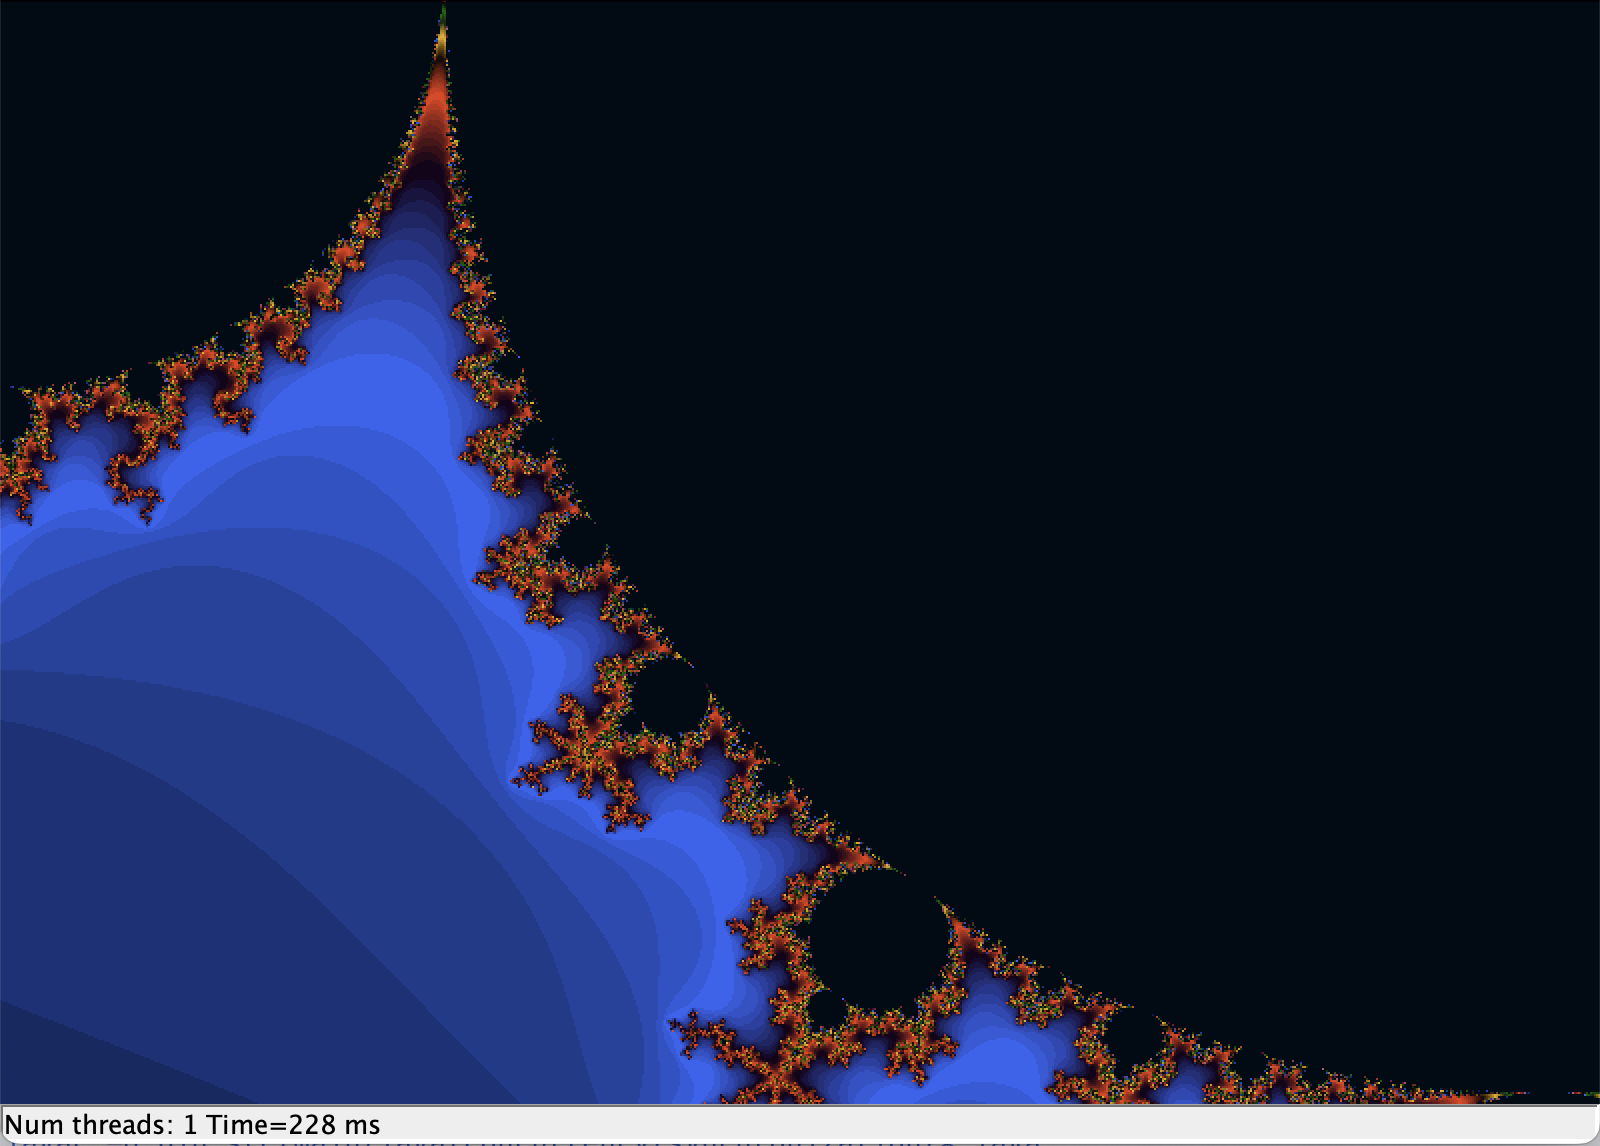
\includegraphics[width=0.6\textwidth]{images/1_thread_3.png} % path to your image
    \caption{Mandelbrot set rendered with 1 thread: 228ms}
    \label{fig:example}
\end{figure}

\begin{figure}[H] % h = place roughly here
    \centering
    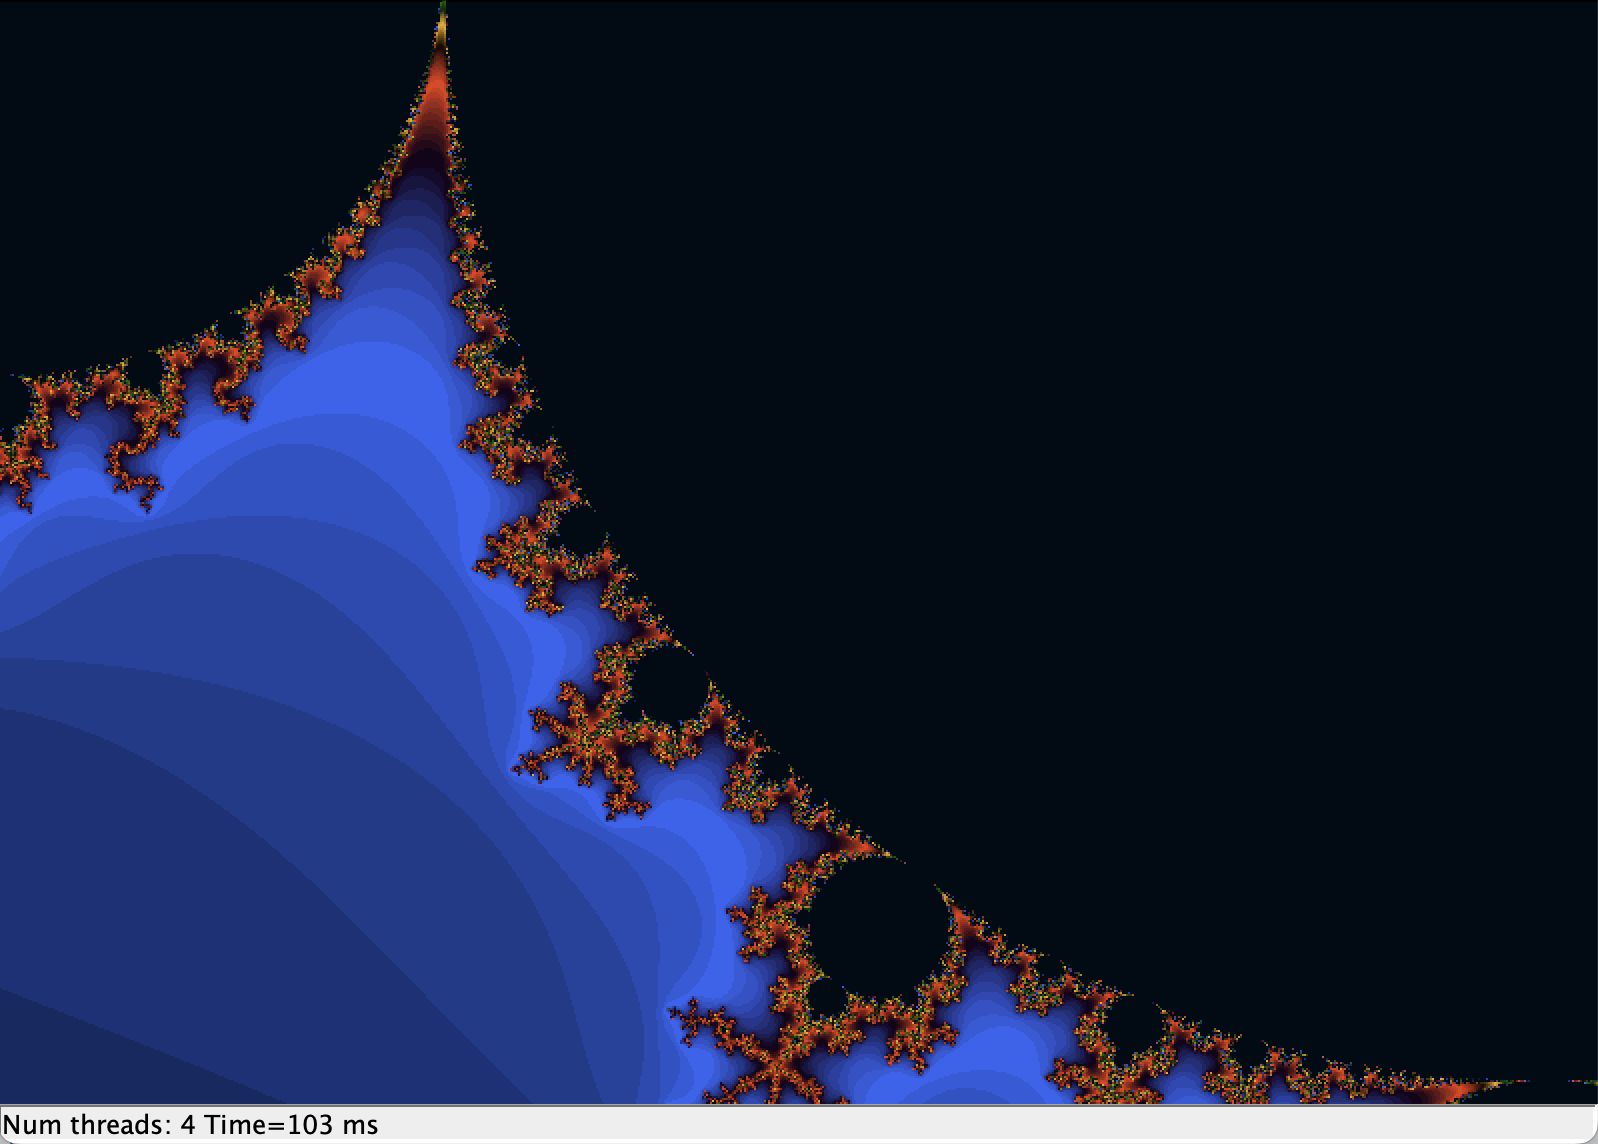
\includegraphics[width=0.6\textwidth]{images/4_threads_3.png} % path to your image
    \caption{Mandelbrot set rendered with 4 threads: 103ms}
    \label{fig:example}
\end{figure}

\end{document}